\documentclass[14pt, a4paper]{article} %14 pt indicates the font size of the prepared document
\usepackage[utf8]{inputenc} %indicates the encoding of the document
\usepackage{multicol}
\usepackage{multirow}
\usepackage{graphicx}
\usepackage{amsmath,esint}

\newcommand*\VF[1]{\mathbf{#1}}
\newcommand*\dif{\mathop{}\!\mathrm{d}}
\usepackage{amsfonts} 
% or 
\usepackage{amssymb}
\usepackage{authblk}
\usepackage{geometry}
\usepackage{subcaption}
\title{CSE 300: Online Assignment}
\author{Md Shamsuzzoha Bayzid, Mahjabin Nahar, Md Shariful Islam Bhuyan and Md Saidur Rahman}

\date{June 2021}

\begin{document}
    \maketitle
    \section{Introduction}
    This assignment has been designed to assess the preparation of the students in writing scientific articles using \LaTeX. This assignment covers a variety of components that are commonly used in scientific manuscripts.
    
    \subsection{Equations}
    Let C be a simple piecewise smooth curve that bounds a region D in the plane. If $P(x, y)$ and $Q(x, y)$ have continuous partials in an open region containing D, then\linebreak
    $\int_C P \,dx + Q \,dy = \iint_D \frac{\partial Q}{\partial x} - \frac{\partial P}{\partial y}$
    \par
    If \textbf{F} is a vector field with third component 0 defined on a domain D enclosed by boundary C then\linebreak
    $
    \oint\limits_C \VF{F}\cdot \,dr
  = \iint\limits_D (\nabla \times \VF{F})\cdot k \dif A
  $
  \par
  Similarly, if C is defined by $\VF{r}(t) = \langle x(t), y(t) \rangle$\linebreak
  $
    \oint\limits_C \VF{F}\cdot \,dx 
  = \iint\limits_D \nabla \cdot \VF{F}\dif A
  $
    \subsection{Tables}
    We wish to place the Table at the bottom of the page.
    
    \subsection{Figures}
    We intend to put Figure \ref{fig:fig1} at the top of the page.
    \pagebreak
    \section{Conclusions}
    The major objectives of this assignment are listed below (please do not ignore the font sizes).
    \begin{itemize}
     \item {\huge{To assess the ability of the students in preparing manuscripts in \LaTeX.}
     }
     \item {\large{ To see if the students have adequately practiced different aspects of writing in \LaTeX.
     }}
     \item{To see if the students can add various basic components (e.g., tables, figures, equations) to a \LaTeX manuscript.
     }
     \item {\small{To see if the students can leverage the available materials (both offline and online) to do something which has not explicitly been taught in the class.
     }}
    \end{itemize}
    \begin{table}[b]
    \centering
    \begin{tabular}{|l||l|l|l|}
    \hline
    \multicolumn{4}{|c|}{Item List} \\ \hline
    Item Name or & \multirow{2}{*}{ALPHA 2 Code} & \multirow{2}{*}{ALPHA 3 Code} & \multirow{2}{*}{Numeric Code} \\ \cline{1-1}
    Product Name &  &  &  \\ \hline
    \multirow{2}{*}{Item001} & \multirow{2}{*}{AF} & \multirow{2}{*}{AFG} & 001 \\
    &  &  & 002 \\ \hline
    Item002 & AX & ALA & 003 \\ \hline
    \multirow{4}{*}{Item003} & \multirow{4}{*}{AL} & \multirow{4}{*}{ALB} & 004 \\
    &  &  & 005 \\
    &  &  & 006 \\
    &  &  & 008 \\ \hline
    \multirow{2}{*}{Item004} & \multirow{2}{*}{DZ} & \multirow{2}{*}{DZA} & 009 \\
    &  &  & 010 \\ \hline
    \multirow{2}{*}{Item005} & \multirow{2}{*}{AS} & \multirow{2}{*}{ASM} & 011 \\
    &  &  & 012 \\ \hline
    Item006 & AD & AND & 013 \\ \hline
    Item007 & AO & AGO & 014 \\ \hline \hline
    \end{tabular}
    \end{table}
    \pagebreak
    \begin{figure}[t]
            \centering
            \begin{subfigure}[b]{0.7\linewidth}
                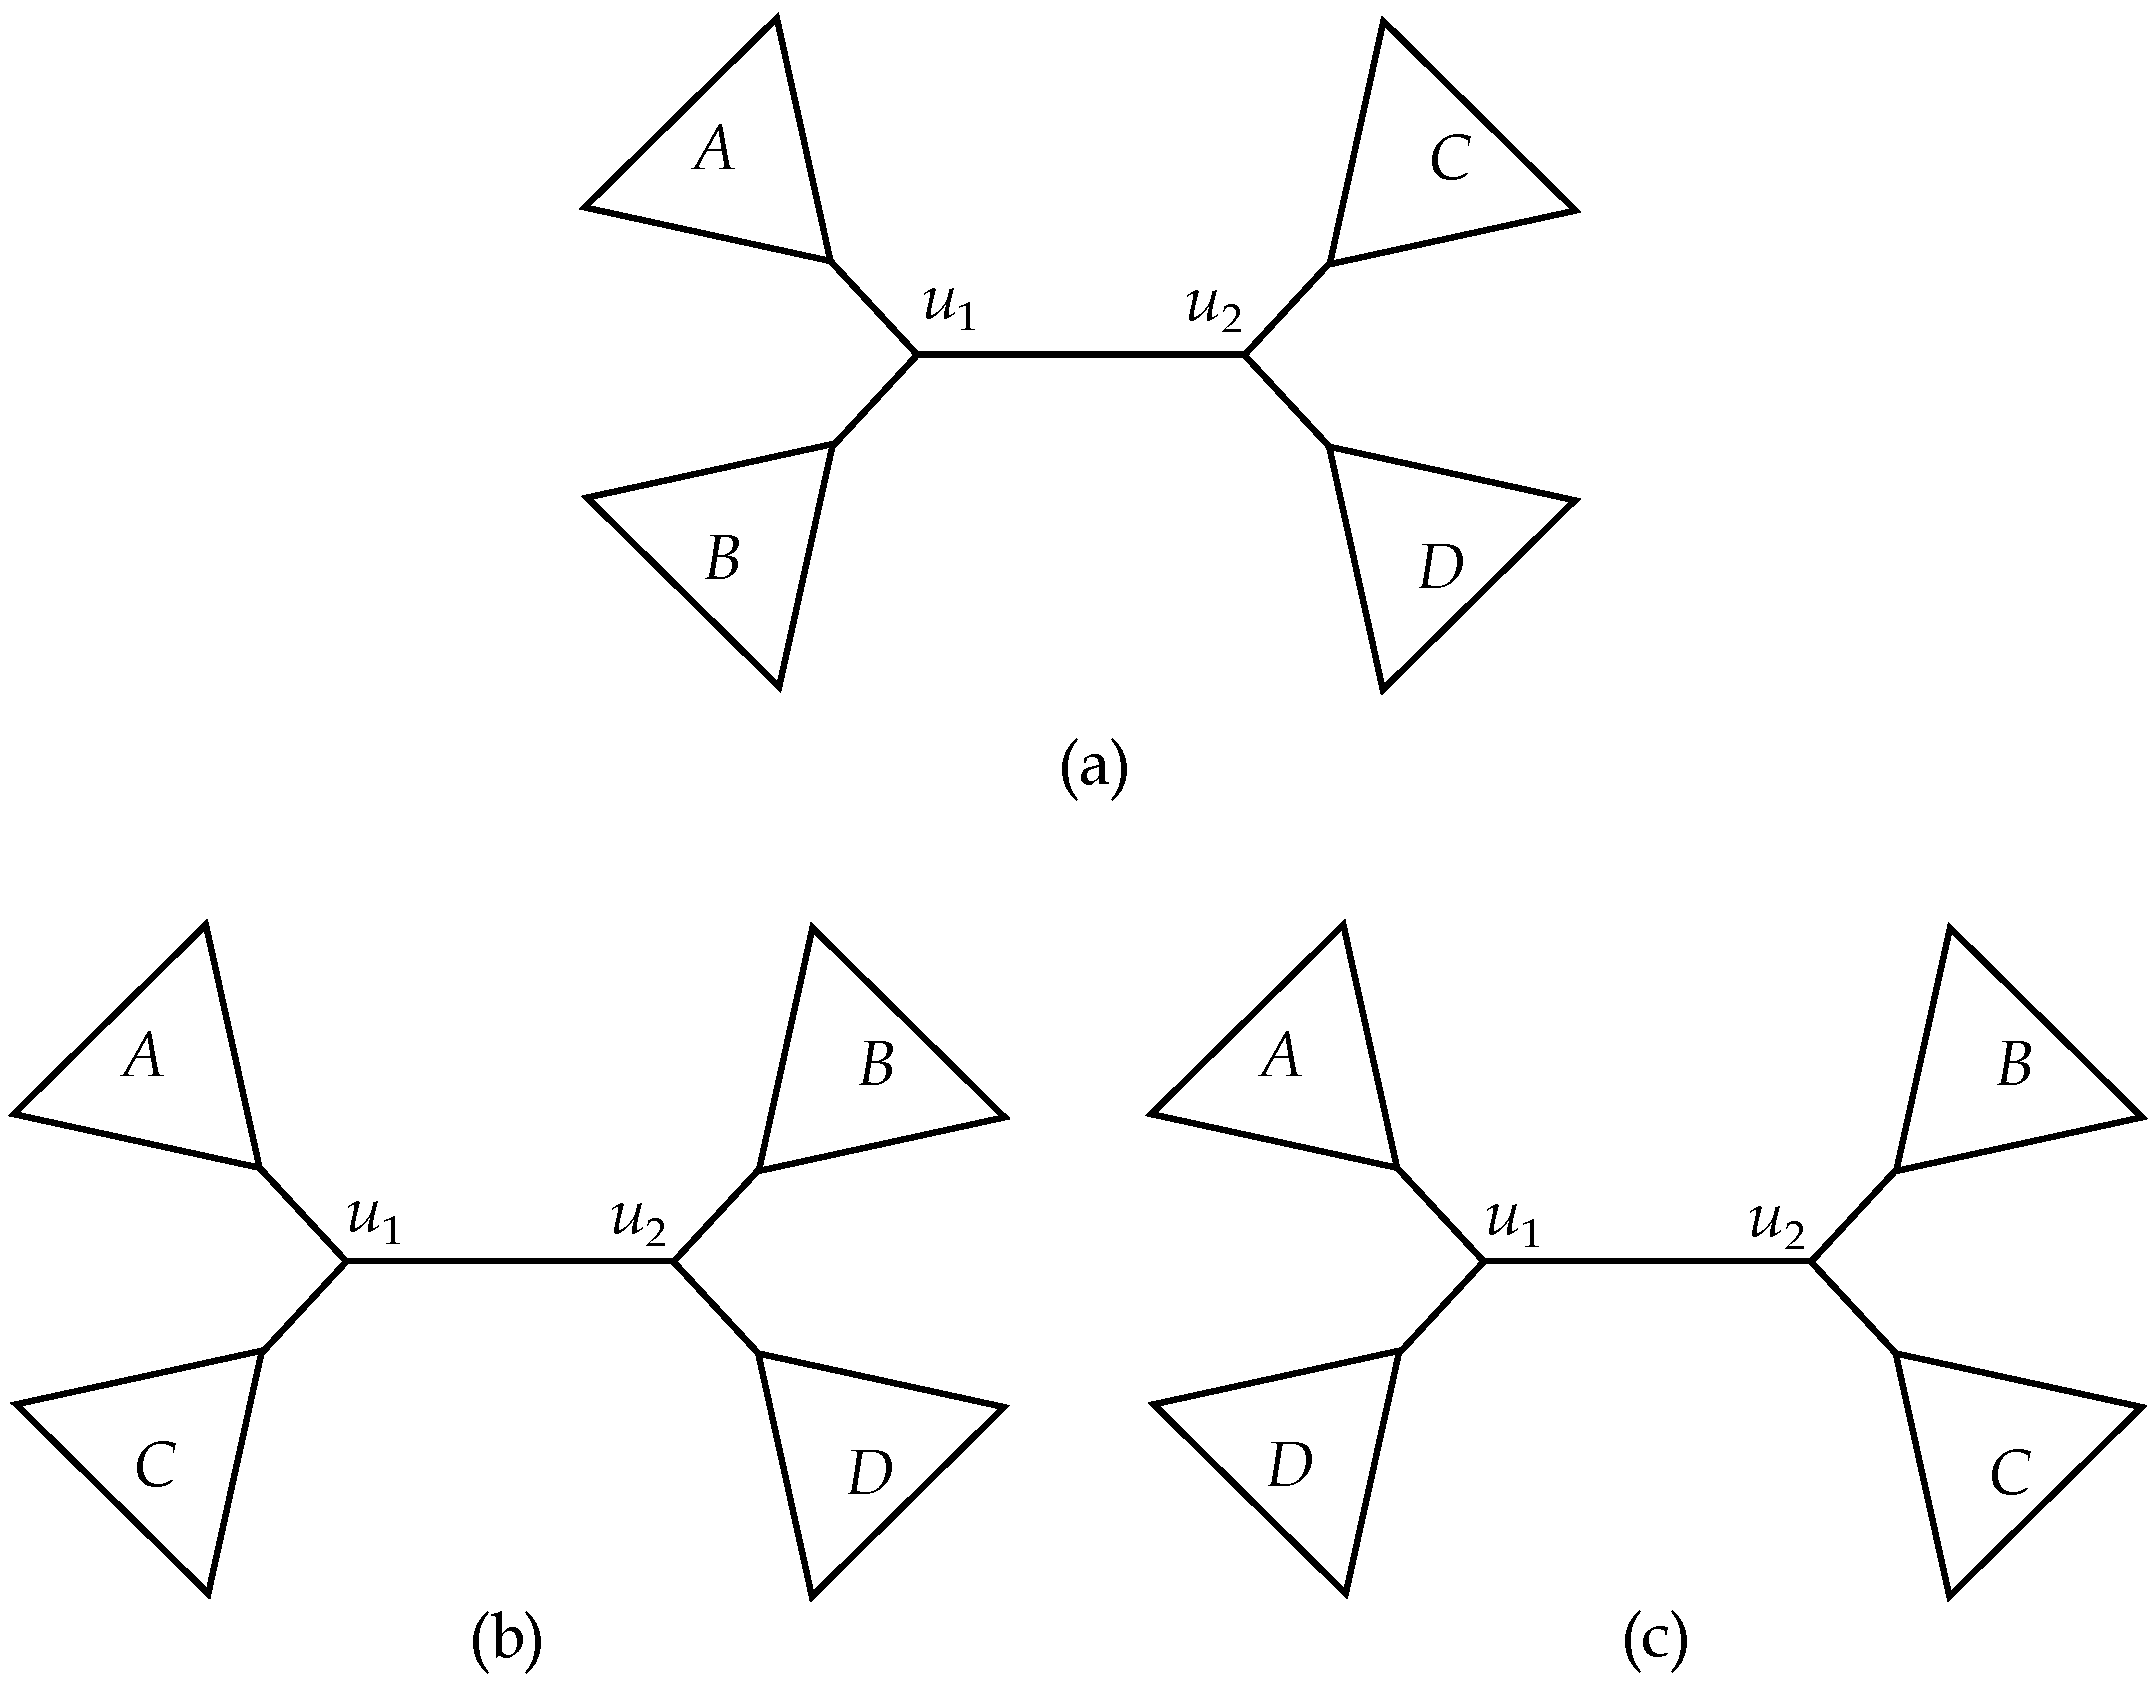
\includegraphics[width=\linewidth, angle=180]{Figure3.pdf}
            \end{subfigure}
            \begin{subfigure}[b]{0.7\linewidth}
                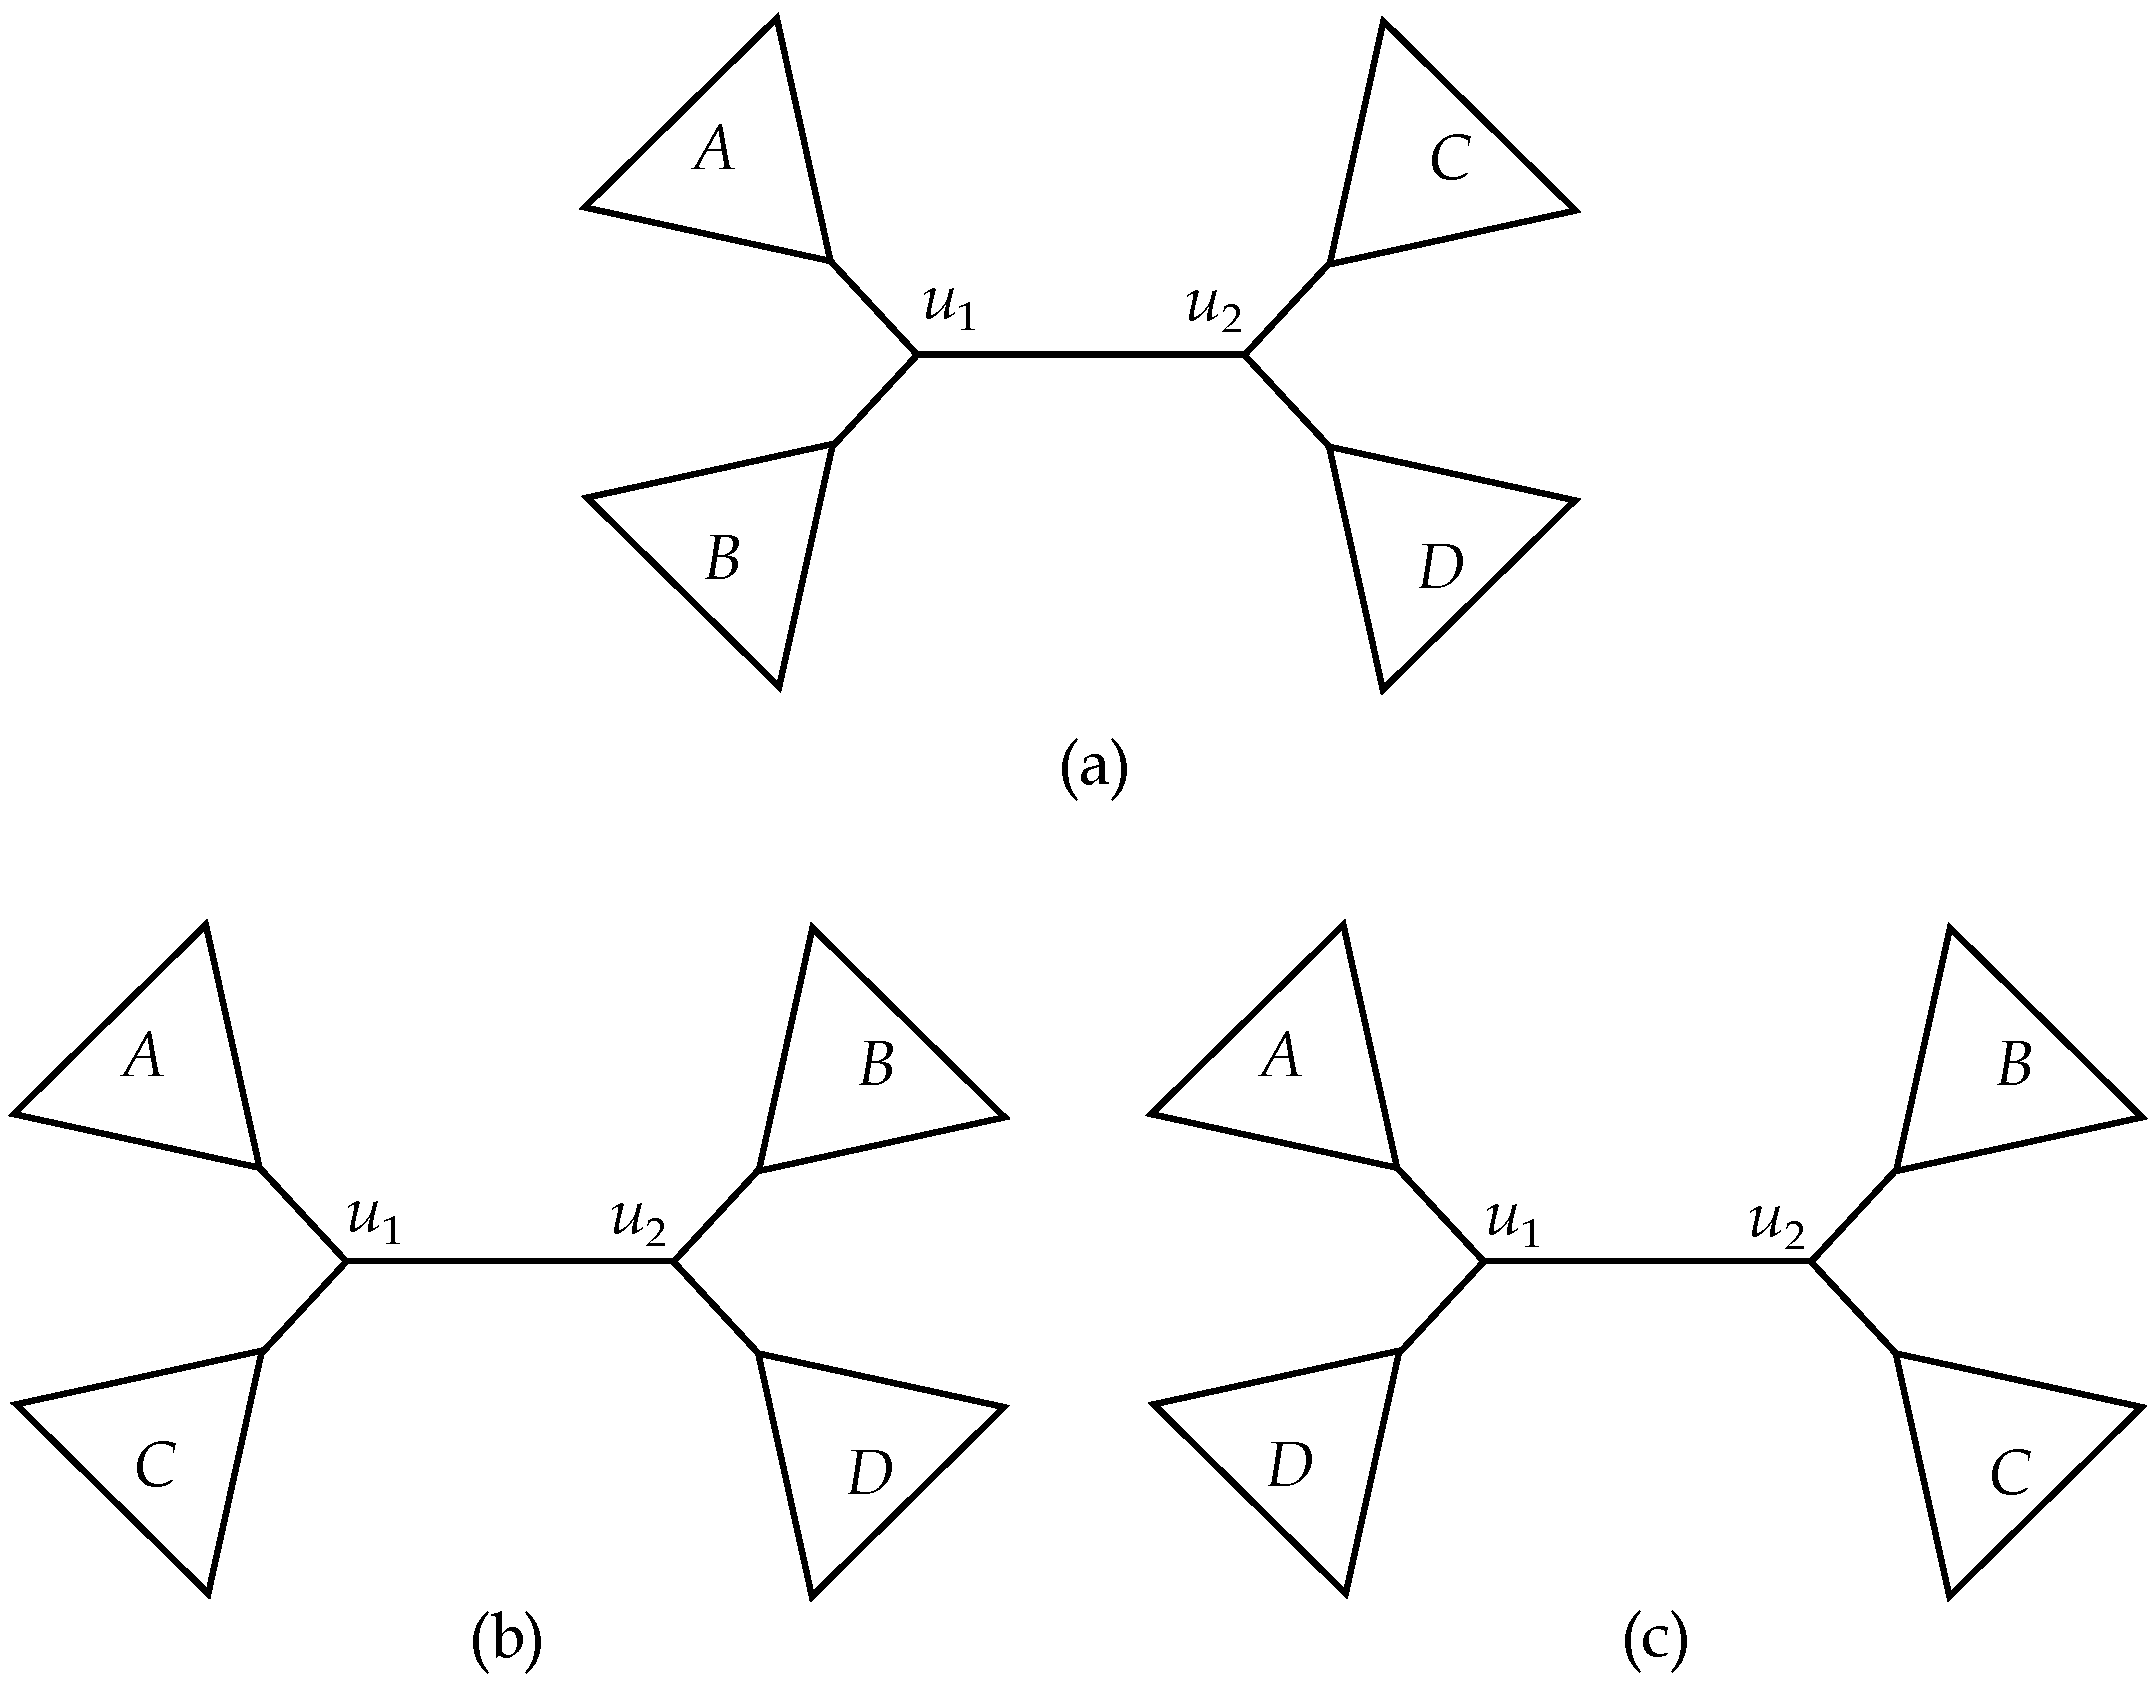
\includegraphics[width=\linewidth]{Figure3.pdf}
            \end{subfigure}
            \caption{\label{fig:fig1}\textbf{Same figure upside down}}
        \end{figure}
\end{document}
